\PassOptionsToPackage{unicode=true}{hyperref} % options for packages loaded elsewhere
\PassOptionsToPackage{hyphens}{url}
%
\documentclass[]{article}
\usepackage{lmodern}
\usepackage{amssymb,amsmath}
\usepackage{ifxetex,ifluatex}
\usepackage{fixltx2e} % provides \textsubscript
\ifnum 0\ifxetex 1\fi\ifluatex 1\fi=0 % if pdftex
  \usepackage[T1]{fontenc}
  \usepackage[utf8]{inputenc}
  \usepackage{textcomp} % provides euro and other symbols
\else % if luatex or xelatex
  \usepackage{unicode-math}
  \defaultfontfeatures{Ligatures=TeX,Scale=MatchLowercase}
\fi
% use upquote if available, for straight quotes in verbatim environments
\IfFileExists{upquote.sty}{\usepackage{upquote}}{}
% use microtype if available
\IfFileExists{microtype.sty}{%
\usepackage[]{microtype}
\UseMicrotypeSet[protrusion]{basicmath} % disable protrusion for tt fonts
}{}
\IfFileExists{parskip.sty}{%
\usepackage{parskip}
}{% else
\setlength{\parindent}{0pt}
\setlength{\parskip}{6pt plus 2pt minus 1pt}
}
\usepackage{hyperref}
\hypersetup{
            pdftitle={First steps with Git},
            pdfauthor={Jakob Willforss},
            pdfborder={0 0 0},
            breaklinks=true}
\urlstyle{same}  % don't use monospace font for urls
\usepackage[margin=1in]{geometry}
\usepackage{color}
\usepackage{fancyvrb}
\newcommand{\VerbBar}{|}
\newcommand{\VERB}{\Verb[commandchars=\\\{\}]}
\DefineVerbatimEnvironment{Highlighting}{Verbatim}{commandchars=\\\{\}}
% Add ',fontsize=\small' for more characters per line
\usepackage{framed}
\definecolor{shadecolor}{RGB}{248,248,248}
\newenvironment{Shaded}{\begin{snugshade}}{\end{snugshade}}
\newcommand{\AlertTok}[1]{\textcolor[rgb]{0.94,0.16,0.16}{#1}}
\newcommand{\AnnotationTok}[1]{\textcolor[rgb]{0.56,0.35,0.01}{\textbf{\textit{#1}}}}
\newcommand{\AttributeTok}[1]{\textcolor[rgb]{0.77,0.63,0.00}{#1}}
\newcommand{\BaseNTok}[1]{\textcolor[rgb]{0.00,0.00,0.81}{#1}}
\newcommand{\BuiltInTok}[1]{#1}
\newcommand{\CharTok}[1]{\textcolor[rgb]{0.31,0.60,0.02}{#1}}
\newcommand{\CommentTok}[1]{\textcolor[rgb]{0.56,0.35,0.01}{\textit{#1}}}
\newcommand{\CommentVarTok}[1]{\textcolor[rgb]{0.56,0.35,0.01}{\textbf{\textit{#1}}}}
\newcommand{\ConstantTok}[1]{\textcolor[rgb]{0.00,0.00,0.00}{#1}}
\newcommand{\ControlFlowTok}[1]{\textcolor[rgb]{0.13,0.29,0.53}{\textbf{#1}}}
\newcommand{\DataTypeTok}[1]{\textcolor[rgb]{0.13,0.29,0.53}{#1}}
\newcommand{\DecValTok}[1]{\textcolor[rgb]{0.00,0.00,0.81}{#1}}
\newcommand{\DocumentationTok}[1]{\textcolor[rgb]{0.56,0.35,0.01}{\textbf{\textit{#1}}}}
\newcommand{\ErrorTok}[1]{\textcolor[rgb]{0.64,0.00,0.00}{\textbf{#1}}}
\newcommand{\ExtensionTok}[1]{#1}
\newcommand{\FloatTok}[1]{\textcolor[rgb]{0.00,0.00,0.81}{#1}}
\newcommand{\FunctionTok}[1]{\textcolor[rgb]{0.00,0.00,0.00}{#1}}
\newcommand{\ImportTok}[1]{#1}
\newcommand{\InformationTok}[1]{\textcolor[rgb]{0.56,0.35,0.01}{\textbf{\textit{#1}}}}
\newcommand{\KeywordTok}[1]{\textcolor[rgb]{0.13,0.29,0.53}{\textbf{#1}}}
\newcommand{\NormalTok}[1]{#1}
\newcommand{\OperatorTok}[1]{\textcolor[rgb]{0.81,0.36,0.00}{\textbf{#1}}}
\newcommand{\OtherTok}[1]{\textcolor[rgb]{0.56,0.35,0.01}{#1}}
\newcommand{\PreprocessorTok}[1]{\textcolor[rgb]{0.56,0.35,0.01}{\textit{#1}}}
\newcommand{\RegionMarkerTok}[1]{#1}
\newcommand{\SpecialCharTok}[1]{\textcolor[rgb]{0.00,0.00,0.00}{#1}}
\newcommand{\SpecialStringTok}[1]{\textcolor[rgb]{0.31,0.60,0.02}{#1}}
\newcommand{\StringTok}[1]{\textcolor[rgb]{0.31,0.60,0.02}{#1}}
\newcommand{\VariableTok}[1]{\textcolor[rgb]{0.00,0.00,0.00}{#1}}
\newcommand{\VerbatimStringTok}[1]{\textcolor[rgb]{0.31,0.60,0.02}{#1}}
\newcommand{\WarningTok}[1]{\textcolor[rgb]{0.56,0.35,0.01}{\textbf{\textit{#1}}}}
\usepackage{graphicx,grffile}
\makeatletter
\def\maxwidth{\ifdim\Gin@nat@width>\linewidth\linewidth\else\Gin@nat@width\fi}
\def\maxheight{\ifdim\Gin@nat@height>\textheight\textheight\else\Gin@nat@height\fi}
\makeatother
% Scale images if necessary, so that they will not overflow the page
% margins by default, and it is still possible to overwrite the defaults
% using explicit options in \includegraphics[width, height, ...]{}
\setkeys{Gin}{width=\maxwidth,height=\maxheight,keepaspectratio}
\setlength{\emergencystretch}{3em}  % prevent overfull lines
\providecommand{\tightlist}{%
  \setlength{\itemsep}{0pt}\setlength{\parskip}{0pt}}
\setcounter{secnumdepth}{0}
% Redefines (sub)paragraphs to behave more like sections
\ifx\paragraph\undefined\else
\let\oldparagraph\paragraph
\renewcommand{\paragraph}[1]{\oldparagraph{#1}\mbox{}}
\fi
\ifx\subparagraph\undefined\else
\let\oldsubparagraph\subparagraph
\renewcommand{\subparagraph}[1]{\oldsubparagraph{#1}\mbox{}}
\fi

% set default figure placement to htbp
\makeatletter
\def\fps@figure{htbp}
\makeatother


\title{First steps with Git}
\author{Jakob Willforss}
\date{2020-10-11}

\begin{document}
\maketitle

\hypertarget{introduction}{%
\section{Introduction}\label{introduction}}

The aim with this tutorial is to get your feet wet with using the Git
terminal to manage your files locally, and to understand how to send
these to GitHub.

To illustrate each step, I am using the visualizations provided by the
web page \href{http://git-school.github.io/visualizing-git/}{Visualizing
Git}. Highly useful for understanding Git and what it does!

\hypertarget{downloading-git}{%
\section{Downloading Git}\label{downloading-git}}

\textbf{NOTE: This is only required if you don't already have
\texttt{git} installed on your computer. You can check this by running
\texttt{git\ -\/-version}. If installed properly, this should give you a
version message.}

\begin{Shaded}
\begin{Highlighting}[]
\FunctionTok{git}\NormalTok{ --version}
\end{Highlighting}
\end{Shaded}

\begin{verbatim}
## git version 2.17.1
\end{verbatim}

\begin{Shaded}
\begin{Highlighting}[]
\BuiltInTok{pwd}
\end{Highlighting}
\end{Shaded}

\begin{verbatim}
## /mnt/4851c27b-0958-480e-8fed-760c8fb94297/Jakob/Projects/jakobwillforss.com/content/post
\end{verbatim}

If installed properly, proceed to \texttt{Creating\ a\ new\ repository}.

If not installed, navigate to \url{https://git-scm.com/} and find the
download for the system you are using. Carry through the installation.

\begin{verbatim}
![Git main site screenshot](/post/2020-10-11-first-steps-with-git.en_files/git_screenshot.png)
\end{verbatim}

\hypertarget{creating-a-new-repository}{%
\section{Creating a new repository}\label{creating-a-new-repository}}

When we start a new project, we start with creating a new folder
(\texttt{mkdir\ PythonHelloProject}). At this point \texttt{Git} is not
involved - we have only created a new folder in our file tree.

We navigate into the folder, and then initialize a new repository using
the command \texttt{git\ init}. This creates a hidden folder
\texttt{.git} inside the \texttt{PythonHelloProject}. Now \texttt{Git}
will track what is happening within this folder.

\begin{Shaded}
\begin{Highlighting}[]
\FunctionTok{mkdir}\NormalTok{ PythonHelloProject}
\BuiltInTok{cd}\NormalTok{ PythonHelloProject}
\FunctionTok{git}\NormalTok{ init}
\end{Highlighting}
\end{Shaded}

\begin{verbatim}
## Initialized empty Git repository in /mnt/4851c27b-0958-480e-8fed-760c8fb94297/Jakob/Projects/jakobwillforss.com/content/post/PythonHelloProject/.git/
\end{verbatim}

\hypertarget{creating-and-adding-your-first-files}{%
\section{Creating and adding your first
files}\label{creating-and-adding-your-first-files}}

Here, we will go through the steps of adding new files to our
repository. This is a three-step procedure:

\begin{enumerate}
\def\labelenumi{\arabic{enumi}.}
\tightlist
\item
  Create a new file in the file tree
\item
  Add the newly created files to the stage, selecting those to include
  in the next commit
\item
  Commit the staged files, creating a snapshot where these files have
  been included
\end{enumerate}

First, we create a Python hello-world script.

\begin{Shaded}
\begin{Highlighting}[]
\BuiltInTok{echo} \StringTok{"#!/usr/bin/env Python3"} \OperatorTok{>}\NormalTok{ hello_python.py}
\BuiltInTok{echo} \StringTok{"print('Hello World!!')"} \OperatorTok{>>}\NormalTok{ hello_python.py}
\end{Highlighting}
\end{Shaded}

Secondly, we also include a README file.

\begin{Shaded}
\begin{Highlighting}[]
\BuiltInTok{echo} \StringTok{"This repository contains Hello-world scripts in different languages"} \OperatorTok{>}\NormalTok{ README.md}
\end{Highlighting}
\end{Shaded}

We can inspect how the files look. At this point, we have simply created
new files on our computer - Git is not involved.

\begin{Shaded}
\begin{Highlighting}[]
\FunctionTok{cat}\NormalTok{ README.md}
\FunctionTok{cat}\NormalTok{ hello_python.py}
\end{Highlighting}
\end{Shaded}

\begin{verbatim}
This repository contains Hello-world scripts in different languages
#!/usr/bin/env Python3
print('Hello World!!')
\end{verbatim}

We can always check with \texttt{git} what is the status of the
repository. Here, we see that Git notices that there are new files
added, which are not part of the current history.

\begin{Shaded}
\begin{Highlighting}[]
\FunctionTok{git}\NormalTok{ status}
\end{Highlighting}
\end{Shaded}

\begin{verbatim}
On branch master

No commits yet

Untracked files:
  (use "git add <file>..." to include in what will be committed)

    README.md
    hello_python.py

nothing added to commit but untracked files present (use "git add" to track)
\end{verbatim}

Let's first add the README file to the history. The first step is to add
the added file to the stage, to prepare it to be committed. (We can add
both files at once, but in more complex cases it is good to keep one
commit per `feature').

\begin{Shaded}
\begin{Highlighting}[]
\FunctionTok{git}\NormalTok{ add README.md}
\end{Highlighting}
\end{Shaded}

When asking Git for the status, now we see that the file is added to the
stage.

\begin{Shaded}
\begin{Highlighting}[]
\FunctionTok{git}\NormalTok{ status}
\end{Highlighting}
\end{Shaded}

\begin{verbatim}
On branch master

No commits yet

Changes to be committed:
  (use "git rm --cached <file>..." to unstage)

    new file:   README.md

Untracked files:
  (use "git add <file>..." to include in what will be committed)

    hello_python.py
\end{verbatim}

We are ready to create a commit, and make new history.

\begin{Shaded}
\begin{Highlighting}[]
\FunctionTok{git}\NormalTok{ commit -m }\StringTok{"first commit"}
\end{Highlighting}
\end{Shaded}

\begin{verbatim}
[master (root-commit) 7d35a90] first commit
 1 file changed, 1 insertion(+)
 create mode 100644 README.md
\end{verbatim}

At this point, our Git history looks the following way:

\begin{verbatim}
![Commit 1](/post/2020-10-11-first-steps-with-git.en_files/2_git_commit1.png)
\end{verbatim}

Next, we add the second file to the stage, preparing it to be commited.

\begin{Shaded}
\begin{Highlighting}[]
\FunctionTok{git}\NormalTok{ add hello_python.py}
\end{Highlighting}
\end{Shaded}

We create a second commit including this file in the history.

\begin{Shaded}
\begin{Highlighting}[]
\FunctionTok{git}\NormalTok{ commit -m }\StringTok{"Add Python-script"}
\end{Highlighting}
\end{Shaded}

\begin{verbatim}
[master 7c8447c] Add Python-script
 1 file changed, 2 insertions(+)
 create mode 100644 hello_python.py
\end{verbatim}

This can be illustrated the following way. Here, the \texttt{HEAD}
points to the version we are looking into, and the \texttt{master} (or
\texttt{main}) points to our main branch.

\begin{verbatim}
![Commit 2](/post/2020-10-11-first-steps-with-git.en_files/3_git_commit2.png)
\end{verbatim}

\hypertarget{updating-existing-files}{%
\section{Updating existing files}\label{updating-existing-files}}

\begin{Shaded}
\begin{Highlighting}[]
\BuiltInTok{echo} \StringTok{"print('That's all, bye!')"} \OperatorTok{>>}\NormalTok{ hello_python.py}
\end{Highlighting}
\end{Shaded}

\begin{Shaded}
\begin{Highlighting}[]
\FunctionTok{git}\NormalTok{ status}
\end{Highlighting}
\end{Shaded}

\begin{verbatim}
On branch master
Changes not staged for commit:
  (use "git add <file>..." to update what will be committed)
  (use "git checkout -- <file>..." to discard changes in working directory)

    modified:   hello_python.py

no changes added to commit (use "git add" and/or "git commit -a")
\end{verbatim}

\begin{Shaded}
\begin{Highlighting}[]
\FunctionTok{git}\NormalTok{ add hello_python.py}
\end{Highlighting}
\end{Shaded}

\begin{verbatim}
![Commit 3](/post/2020-10-11-first-steps-with-git.en_files/4_git_commit3.png)
\end{verbatim}

\hypertarget{moving-back-and-forth-in-history}{%
\section{Moving back and forth in
history}\label{moving-back-and-forth-in-history}}

One of the powerful features of Git is that we at any point can go back
to any previous snapshots. By doing this, the \texttt{file\ tree} (the
files we see on our computer) changes into the state the files were in
at that point. This allows us to, for instance, explore how our scripts
looked before introducing bugs.

\begin{figure}
\centering
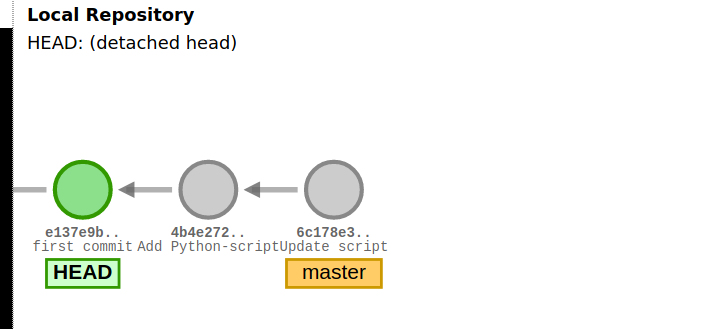
\includegraphics{/post/2020-10-11-first-steps-with-git.en_files/5_git_checkout.png}
\caption{Git checkout}
\end{figure}

We can at any point navigate back to the latest commit by using the
command \texttt{git\ checkout} and specifying the head of the branch
(either \texttt{master} or \texttt{main}).

\begin{Shaded}
\begin{Highlighting}[]
\FunctionTok{git}\NormalTok{ checkout master}
\end{Highlighting}
\end{Shaded}

\begin{verbatim}
Already on 'master'
M   hello_python.py
\end{verbatim}

\begin{figure}
\centering
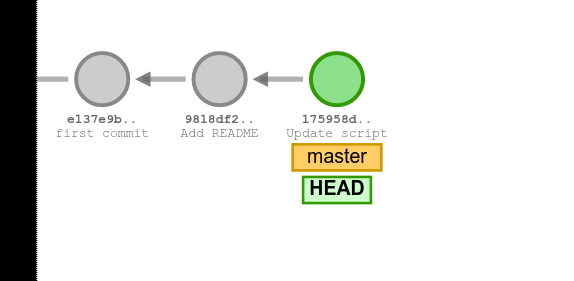
\includegraphics{/post/2020-10-11-first-steps-with-git.en_files/4_git_commit3.png}
\caption{Commit 3}
\end{figure}

\hypertarget{sending-a-repository-to-github}{%
\section{Sending a repository to
GitHub}\label{sending-a-repository-to-github}}

Setup a new repository on GitHub. Give it a name, and assign it as
public. Don't add the README this time! (As you already have created
one.)

{[}img{]}

You will come to a page similar to the following. Follow the
instructions for `push an existing repository from the command line'

{[}log{]}

Note: ssh vs http

\begin{Shaded}
\begin{Highlighting}[]
\NormalTok{git remote add origin XXX}
\NormalTok{git branch }\OperatorTok{-}\NormalTok{M main}
\NormalTok{git push }\OperatorTok{-}\NormalTok{u origin main}
\end{Highlighting}
\end{Shaded}

\hypertarget{concluding-words}{%
\section{Concluding words}\label{concluding-words}}

This only provides a `teaser' for the functionality of Git. By putting
some more time into working through a workshop, you will have a powerful
and useful tool at your disposal. I would strongly encourage you to
start using Git in your next coding- or analysis-project, and gradually
get used to it. When proficient, you will have the full benefit of Git
with very little effort.

Some resources for further reading:

\begin{itemize}
\tightlist
\item
  My materials
\item
  Link 2
\item
  Link 3
\item
  Link 4
\end{itemize}

\end{document}
